\documentclass{beamer}

\usepackage[utf8]{inputenc}
\usepackage[T1]{fontenc} % Allows bold italic text in title

%\usetheme{Berlin}
%\usecolortheme{spruce}

\usetheme[progressbar=frametitle]{metropolis}
\setbeamertemplate{frame numbering}[fraction]
\useoutertheme{metropolis}
\useinnertheme{metropolis}
\usefonttheme{metropolis}
\usecolortheme{spruce}
\setbeamercolor{background canvas}{bg=white}

%\setbeamertemplate{section in toc}[ball unnumbered]
%\setbeamertemplate{subsection in toc}[ball unnumbered]
\setbeamertemplate{section in toc}[sections numbered]
\setbeamertemplate{subsection in toc}[subsections numbered]

\title{Al Loro: \\Lector de \textit{feeds RSS} para asistente de voz}
\author[Alejandro Gómez Noé]{\emph{Autor:} Alejandro Gómez Noé\\[0.3em]\emph{Tutor:} Vicente Pelechano Ferragud}
\institute{ETSINF - Universidad Politécnica de Valencia}
\date{Curso 2020-2021}

\begin{document}
  
  \begin{frame}
    \titlepage
  \end{frame}
  
  \begin{frame}{Índice general}
    \tableofcontents
  \end{frame}

  \section{Introducción}
 
  \begin{frame}{¿Qué es Alexa?}
    \begin{columns}[c]
      \begin{column}{.51\textwidth}
        \begin{itemize}
          \setlength\itemsep{1.5em}
          \only<1>
          {
          \item Alexa es un \textbf{asistente de voz}
          \item Es un servicio de \textbf{Amazon}
          \item Puede obtener información como el \textbf{tiempo}, el \textbf{tráfico}, o las \textbf{noticias}
          }
          \only<2>
          {
          \item Disponible en \textbf{dispositivos Echo} y \textbf{móviles}
          \item Integración con \textbf{domótica}
          \item Permite a los desarrolladores crear \textbf{aplicaciones} (\textbf{\emph{skills}})
          }
        \end{itemize}
      \end{column}
      \begin{column}{.49\textwidth}
        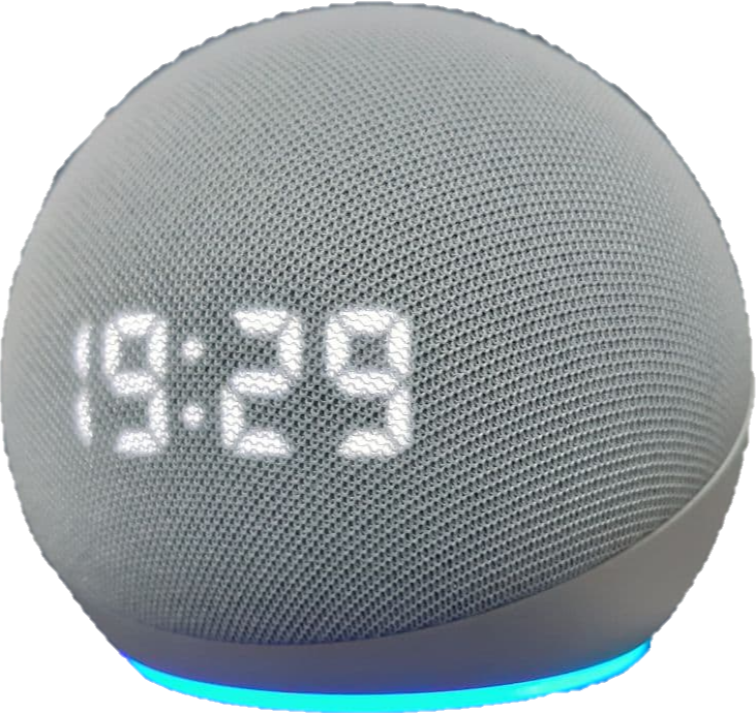
\includegraphics[width=.46\textwidth]{echo-dot.png}
        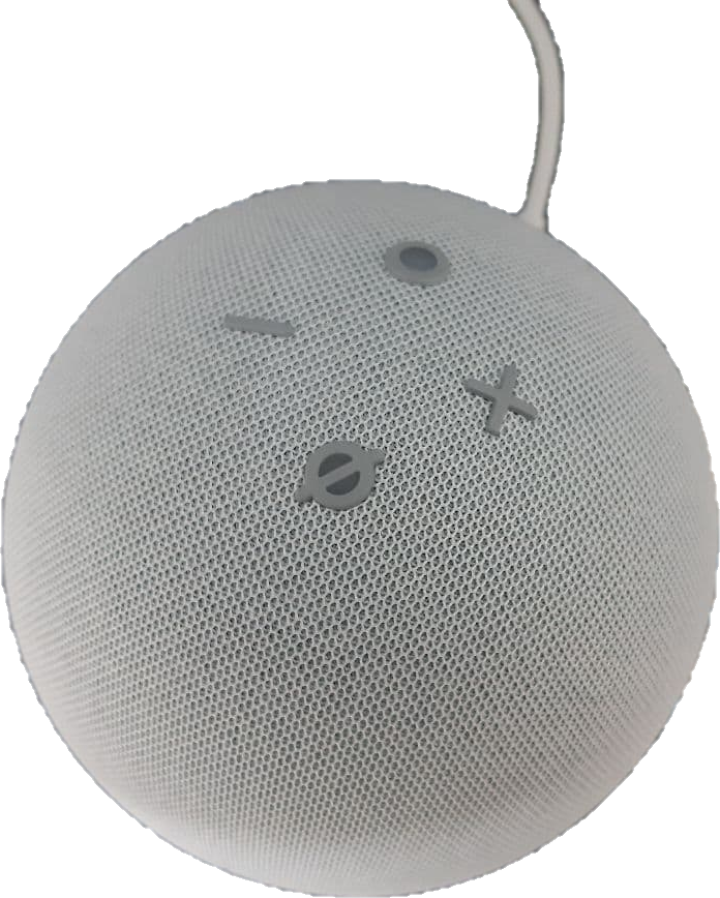
\includegraphics[width=.46\textwidth]{echo-dot-2.png}
        \centering \vspace{0.5em}
        
        \footnotesize
        Dispositivo Amazon Echo Dot\\
        (4ª Generación, con reloj)
      \end{column}
    \end{columns}
  \end{frame}

  \section{Motivación}

  \newcommand{\includecenteredgraphics}[2]{\hspace{.1em}\raisebox{-.39\height}{\includegraphics[scale=#1]{#2}}}
 
  \begin{frame}{Motivación}
    \begin{itemize}
      \setlength\itemsep{1.5em}
      \item Entender más sobre los \textbf{servicios en la nube}
      \includecenteredgraphics{.35}{aws-lambda-logo.png}
      \item Aprender un lenguaje de programación (\textbf{TypeScript})
      \includecenteredgraphics{.02}{typescript-logo.png}
      \item Introducirme en un campo nuevo (\textbf{asistentes de voz})
      \includecenteredgraphics{.09}{amazon-alexa.png}
    \end{itemize}
  \end{frame}

  \section{Estado del arte}
  
  \section{Propuesta de solución}
  
  \section{Diseño, arquitectura, esquema de la solución realizada}
  
  \section{Desarrollo / Implementación de la propuesta}
  
  \section{Demo}
  
  \section{Resultados obtenidos}
  
  \section{Conclusiones} % (y trabajos futuros)

\end{document}